\documentclass[12pt]{article}

\usepackage[a4paper,margin=2cm]{geometry}

\usepackage{amsmath}
\usepackage{amssymb}
\usepackage{mathtools}

\usepackage{listings}

\usepackage{booktabs} % For tables
\usepackage[table,xcdraw]{xcolor} % For tables

\usepackage{tikz} % TikZ

\usepackage{enumerate}
\usepackage{enumitem}

\usepackage{nameref}

\usepackage{xcolor}

\definecolor{codegreen}{rgb}{0,0.6,0}
\definecolor{codegray}{rgb}{0.5,0.5,0.5}
\definecolor{codepurple}{rgb}{0.58,0,0.82}
\definecolor{backcolour}{rgb}{0.95,0.95,0.92}

\lstdefinestyle{mystyle}{
    backgroundcolor=\color{backcolour},
    commentstyle=\color{codegreen},
    keywordstyle=\color{magenta},
    numberstyle=\tiny\color{codegray},
    stringstyle=\color{codepurple},
    basicstyle=\ttfamily\footnotesize,
    breakatwhitespace=false,
    breaklines=true,
    captionpos=b,
    keepspaces=true,
    numbers=left,
    numbersep=5pt,
    showspaces=false,
    showstringspaces=false,
    showtabs=false,
    tabsize=2
}

\lstset{style=mystyle}

\DeclarePairedDelimiter\abs{\lvert}{\rvert}
\DeclarePairedDelimiter\Abs{\lVert}{\rVert}

\usepackage{fancyhdr}

\pagestyle{fancy}
\lhead{\today}
\chead{Exercise 04\\Algorithmic Foundations of Data Science}
\rhead{Fabian Grob\\Simon Michau\\Til Mohr}

\setlength{\headheight}{50pt}

\begin{document}

\section*{Exercise 1}
\subsection*{(a)}
Situation for l=2 and s=2:
\[Q_{2,2}=\lbrace [x_1 x_2]^T\in\mathbb{R}^2\mid |x_i|\leq 1 \text{ for all } i=1,2\rbrace = [-1,1]^2\]
\begin{center}
	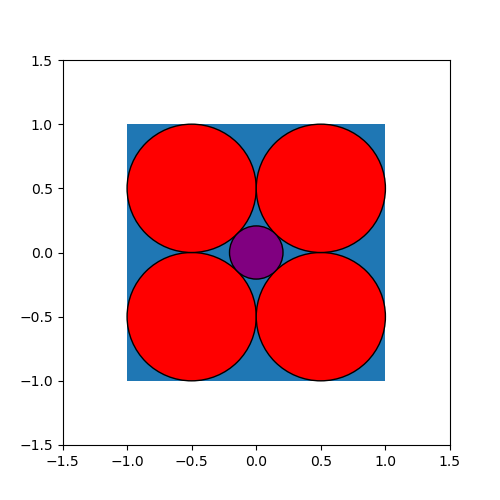
\includegraphics[width=3.5in]{code/exercise_01_a.png}
\end{center}

\subsection*{(b)}
First, let's calculate the radius of the inner hyperball for any $l \in \mathbb{N}, s \in \mathbb{R}_{>0}$: \\
The distance from the center of the inner hyperball (equal to the center of the hypercube) to the center of one of the $2^l$ outter hyperballs (doesn't matter which one) can be calculated the following:
\begin{equation*}
	d \coloneqq \sqrt{l \cdot \left( \frac{s}{4} \right)^2}
\end{equation*}
Thus, the radius of the inner hyperball is equal to:
\begin{equation*}
	r \coloneqq d - \frac{s}{4} = \sqrt{l \cdot \left( \frac{s}{4} \right)^2} - \frac{s}{4}
\end{equation*}
Now, we simply must solve the following inequality to find an $l \in \mathbb{N}$ for an arbitrary but fixed $s \in \mathbb{R}_{>0}$ such that $B(Q_{l,s}) \not\subseteq Q_{l,s}$:
\begin{align*}
	\frac{s}{2} &< r \\
	\frac{s}{2} &< d - \frac{s}{4} \\
	\frac{s}{2} &< \sqrt{l \cdot \left( \frac{s}{4} \right)^2} - \frac{s}{4} \\
	\frac{3 \cdot s}{4} &< \sqrt{l} \cdot \frac{s}{4} \\
	3 &< \sqrt{l} \\
	l &> 9
\end{align*}

\section*{Exercise 2}
\subsection*{(a)}
Let's first find all eigenvalues of $A_c$:
\begin{align*}
	\{ \lambda \in \mathbb{R} &\mid \det\left( A_c - \lambda \cdot I_3 \right) = 0\} \\
	\{ \lambda \in \mathbb{R} &\mid \det\left[ \begin{array}{ccc} 2 - \lambda & 0 & c \\ 0 & 1 - \lambda & 0 \\ c & 0 & 1 - \lambda \end{array} \right] = 0\} \\
	\{ \lambda \in \mathbb{R} &\mid -\lambda^3 + 4 \cdot \lambda^2 + c^2 \cdot \lambda - 5 \cdot \lambda + 2 -c^2\} \\
	\{ \lambda \in \mathbb{R} &\mid (\lambda - 1) \cdot (-\lambda^2 + 3 \dot \lambda + c^2 - 2)\} \\
	\{ 1, \frac{3 - \sqrt{4 \cdot c^2 + 1}}{2}, \frac{3 + \sqrt{4 \cdot c^2 + 1}}{2}\} \eqqcolon \Lambda_{A_c}\\
\end{align*}
So, if for all $\lambda \in \Lambda_{A_c}$ it must hold that $\lambda \geq 0$, we must set $c$ such that the following inequality holds:
\begin{align*}
	\frac{3 - \sqrt{4 \cdot c^2 + 1}}{2} &\geq 0 \\
	3 - \sqrt{4 \cdot c^2 + 1} &\geq 0 \\
	3 &\geq \sqrt{4 \cdot c^2 + 1} \\
	9 &\geq 4 \cdot c^2 + 1 \\
	8 &\geq 4 \cdot c^2 \\
	2 &\geq c^2 \\
	c \in (-\sqrt{2}&, \sqrt{2}) \subseteq \mathbb{R}
\end{align*}

\subsection*{(b)}
Using Theorem 5.19, we create an orthogonal matrix $U \in \mathbb{R}^{n \times n}$ with the columns being the eigenvectors of $A$. We can now use Theorem 5.20 to create the diagonal matrix $\Lambda \in \mathbb{R}^{n \times n}$ where the eigenvalue-entry $\lambda_{i,i}$ corresponds to eigenvector in the column $i$ of $U$. \\
A simple verification:
\begin{align*}
	A &= U \Lambda U^\top \\
	A &= U \Lambda U^{-1} \\
	A U &= U \Lambda \\
	A v_i &= v_i \lambda_{i,i} \qquad, \forall i \in \left[n\right], v_i \coloneqq col_i(U) \\
	A v_i &= \lambda_{i,i} v_i \qquad, \forall i \in \left[n\right], v_i \coloneqq col_i(U) \\
\end{align*}
Since $A$ is positive semi-definite, all entries $\lambda_{i,i} \geq 0$. Thus, we can create a diagonal matrix $\Lambda'$ consisting of the entries $\lambda'_{i,i} \coloneqq \sqrt{\lambda_{i,i}}$. Thus, $\Lambda = \Lambda' \Lambda'^\top$. Let $B \coloneqq U U \Lambda'$. Now:
\begin{align*}
	A &= U \Lambda U^\top \\
	A &= U (\Lambda' \Lambda'^\top) U^\top \\
	A &= U (\Lambda' \Lambda'^\top) U^\top \\
	A &= (U \Lambda') (\Lambda'^\top U^\top) \\
	A &= (U \Lambda') (U \Lambda')^\top \\
	A &= B B^\top \\
\end{align*}

\subsection*{(c)}
Since $A$ is symmetric, the following holds $\forall x,y \in R^n$:
\begin{equation*}
	\langle Ax,y \rangle = \langle x,Ay \rangle
\end{equation*}
Let $v_1 \in E_1, v_2 \in E_2$. Then $A v_1 = \lambda_1 v_1$ and $A v_2 = \lambda_2 v_2$.
\begin{align*}
	0 &= \langle Av_1,v_2 \rangle - \langle v_1,Av_2 \rangle \\
	&= \langle \lambda_1v_1,v_2 \rangle - \langle v_1,\lambda_2v_2 \rangle \\
	&= (\lambda_1 - \lambda_2) \langle v_1,v_2 \rangle \\
\end{align*}
Since $\lambda_1 \neq \lambda_2$ it follows, that $\langle v_1,v_2 \rangle = 0$.

\section*{Exercise 3}
\subsection*{(a)}
Plot and estimate first principal component $(\frac{1}{\sqrt{5}}, \frac{2}{\sqrt{5}})$
\begin{center}
	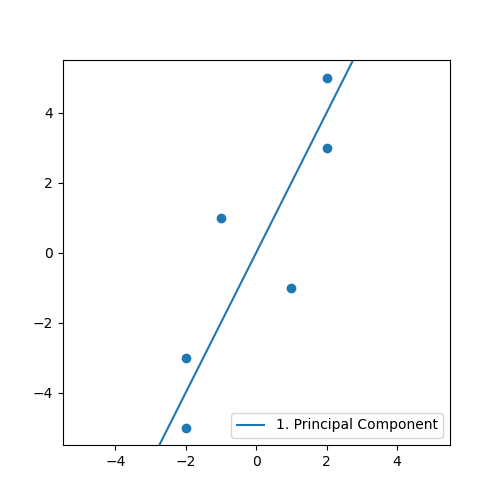
\includegraphics[width=3.5in]{code/exercise_03_a.png}
\end{center}

\subsection*{(b)}
\begin{align*}
	C &\coloneqq A^\top A \\
	&= \left[ \begin{array}{cccccc}
		-2 & -2 & -1 & 1 & 2 & 2 \\
		-5 & -3 & 1 & 1 & 3 & 5
	\end{array} \right] \left[ \begin{array}{cc}
		-2 & -5 \\
		-2 & 3 \\
		-1 & 1 \\
		1 & -1 \\
		2 & 3 \\
		2 & 5
	\end{array} \right] \\
	&= \left[ \begin{array}{cc}
		18 & 18 \\
		18 & 70
	\end{array} \right]
\end{align*}

\subsection*{(c)}
View code in the appendix for the calculations. \\
The eigenvector we got is: $\left( \begin{array}{c} 0.298 \\ 0.954 \end{array}\right)$

\subsection*{(d)}
Well, they both point in the same general direction with a slope greater than 1. Our slope came out to be at $2$, since eye-balling stuff tends to round to integer values. The more optimal slope however seems to be even greater than $3 < \frac{0.954}{0.298}$.

\section*{Exercise 4}
\subsection*{(a)}
\begin{equation*}
	S \coloneqq \left[
	\begin{array}{cccccccc}
		0 & 0 & 1 & 1 & 1 & 0 & 0 & 0 \\
		0 & 0 & 1 & 1 & 0 & 0 & 0 & 0 \\
		1 & 1 & 0 & 1 & 0 & 0 & 0 & 0 \\
		1 & 1 & 1 & 0 & 0 & 0 & 0 & 1 \\
		1 & 0 & 0 & 0 & 0 & 1 & 1 & 1 \\
		0 & 0 & 0 & 0 & 1 & 0 & 1 & 1 \\
		0 & 0 & 0 & 0 & 1 & 1 & 0 & 0 \\
		0 & 0 & 0 & 1 & 1 & 1 & 0 & 0
	\end{array} \right]
\end{equation*}

\begin{equation*}
	D \coloneqq \left[
	\begin{array}{cccccccc}
		3 & 0 & 0 & 0 & 0 & 0 & 0 & 0 \\
		0 & 2 & 0 & 0 & 0 & 0 & 0 & 0 \\
		0 & 0 & 3 & 0 & 0 & 0 & 0 & 0 \\
		0 & 0 & 0 & 4 & 0 & 0 & 0 & 0 \\
		0 & 0 & 0 & 0 & 4 & 0 & 0 & 0 \\
		0 & 0 & 0 & 0 & 0 & 3 & 0 & 0 \\
		0 & 0 & 0 & 0 & 0 & 0 & 2 & 0 \\
		0 & 0 & 0 & 0 & 0 & 0 & 0 & 3
	\end{array} \right]
\end{equation*}

\begin{equation*}
	L \coloneqq D - S = \left[
	\begin{array}{cccccccc}
		3 & 0 & -1 & -1 & -1 & 0 & 0 & 0 \\
		0 & 2 & -1 & -1 & 0 & 0 & 0 & 0 \\
		-1 & -1 & 3 & -1 & 0 & 0 & 0 & 0 \\
		-1 & -1 & -1 & 4 & 0 & 0 & 0 & -1 \\
		-1 & 0 & 0 & 0 & 4 & -1 & -1 & -1 \\
		0 & 0 & 0 & 0 & -1 & 3 & -1 & -1 \\
		0 & 0 & 0 & 0 & -1 & -1 & 2 & 0 \\
		0 & 0 & 0 & -1 & -1 & -1 & 0 & 3
	\end{array} \right]
\end{equation*}

\subsection*{(b)}
View code in the appendix for the calculations. \\
\begin{align*}
	\lambda_1 &= 0.0 \\
	u_1 &= \left( \begin{array}{c}
		-0.354 \\ 0.169 \\ -0.408 \\ 0.408 \\ 0.548 \\ -0.214 \\ 0.408 \\ -0.002
	\end{array} \right) \\
	\lambda_2 &= 0.657 \\
	u_2 &= \left( \begin{array}{c}
		-0.354 \\ 0.493 \\ -0.149 \\ -0.558 \\ -0.358 \\ 0.056 \\ 0.408 \\ -0.002
	\end{array} \right)
\end{align*}

\subsection*{(c)}
The eigenvalue $\lambda_1$ is extremely close to 0. Therefore, $\lambda_1 u_1$ is very close to 0, so also $A u_1$ must be very close to 0.

\subsection*{(d)}
\begin{center}
	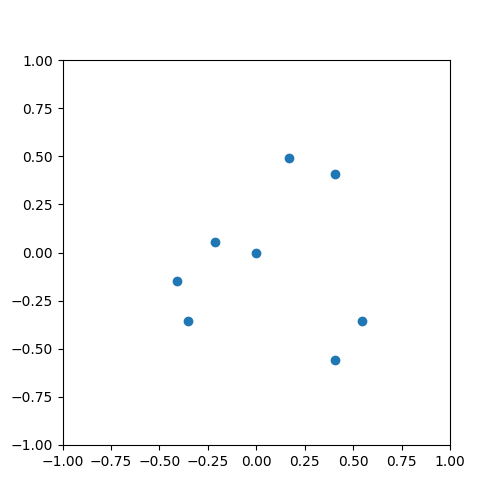
\includegraphics[width=3.5in]{code/exercise_04_d.png}
\end{center}

\subsection*{(e)}
The Spectral Clustering Algorithm returns the clusters computed using the k-means clustering algorithm on the points $\left( (u_1)_i, (u_2)_i \right), i = 1, \dots, 8$. Therefore, depending on the starting centroids, we might see a cluster containing only the two bottom right points, and another containing the remaining points.

\section*{Exercise 5}
\begin{center}
	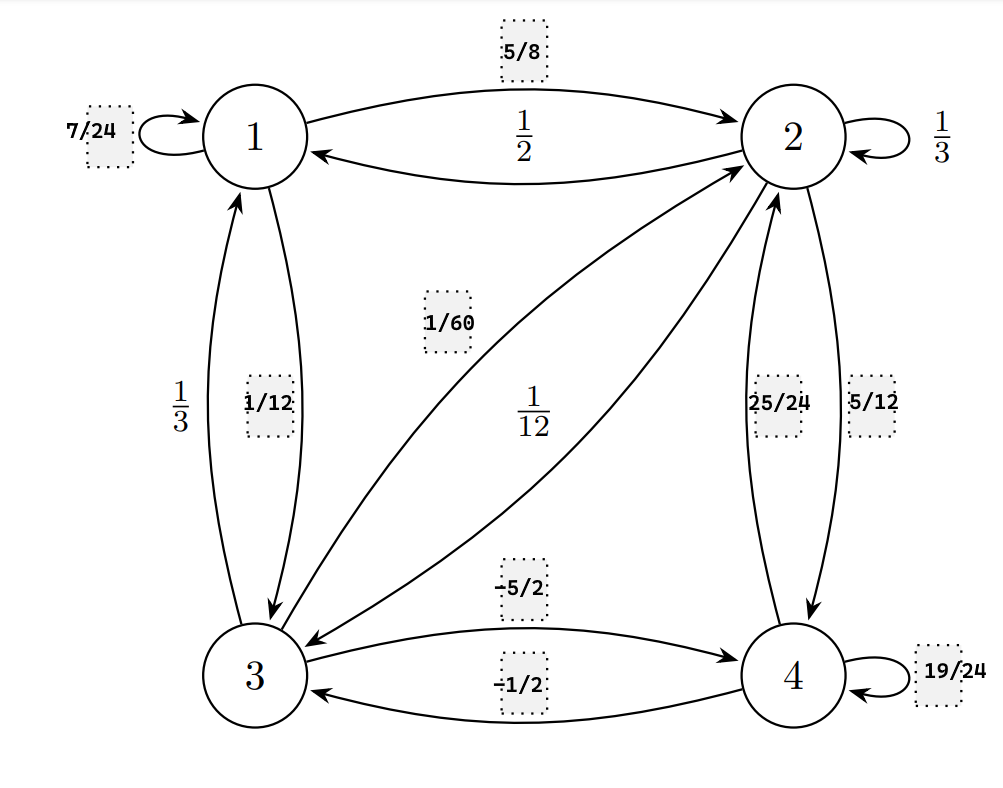
\includegraphics[width=\textwidth]{code/exercise_05.png}
\end{center}

\begin{align*}
	\pi_1 &= \pi_1 q_{11} + \pi_2 q_{21} + \pi_3 q_{31} \\
	\frac{4}{12} &= \frac{4}{12} q_{11} + \frac{5}{12} \frac{1}{2} + \frac{1}{12} \frac{1}{3} \\
	4 &= 4 q_{11} + 5 \frac{1}{2} + 1 \frac{1}{3} \\
	4 &= 4 q_{11} + \frac{17}{6} \\
	\frac{7}{6} &= 4 q_{11} \\
	q_{11} &= \frac{7}{24}
\end{align*}

\begin{align*}
	\pi_1 q_{12} &= \pi_2 q_{21} \\
	\frac{4}{12} q_{12} &= \frac{5}{12} \frac{1}{2} \\
	4 q_{12} &= 5 \frac{1}{2} \\
	q_{12} &= \frac{5}{8}
\end{align*}

\begin{align*}
	\pi_1 q_{13} &= \pi_3 q_{31} \\
	\frac{4}{12} q_{13} &= \frac{1}{12} \frac{1}{3} \\
	4 q_{13} &= \frac{1}{3} \\
	q_{13} &= \frac{1}{12}
\end{align*}

\begin{align*}
	\pi_2 q_{23} &= \pi_3 q_{32} \\
	\frac{5}{12} q_{23} &= \frac{1}{12} \frac{1}{12} \\
	5 q_{23} &= \frac{1}{12} \\
	q_{23} &= \frac{1}{60}
\end{align*}

\begin{align*}
	\pi_2 &= \pi_1 q_{12} + \pi_2 q_{22} + \pi_3 q_{32} + \pi_4 q_{42} \\
	\frac{5}{12} &= \frac{4}{12} \frac{7}{24} + \frac{5}{12} \frac{1}{3} + \frac{1}{12} \frac{1}{12} + \frac{2}{12} q_{42} \\
	5 &= 4 \frac{7}{24} + 5 \frac{1}{3} + 1 \frac{1}{12} + 2 q_{42} \\
	5 &= \frac{35}{12} + 2 q_{42} \\
	\frac{25}{12} &= 2 q_{42} \\
	q_{42} &= \frac{25}{24}  \\
\end{align*}

\begin{align*}
	\pi_2 q_{24} &= \pi_4 q_{42} \\
	\frac{5}{12} q_{24} &= \frac{2}{12} \frac{25}{24} \\
	5 q_{24} &= 2 \frac{25}{24} \\
	q_{24} &= \frac{5}{12}
\end{align*}

\textbf{THIS MUST BE WRONG FOR SURE: $q_{43}$ cannot be negative, I believe}

\begin{align*}
	\pi_3 &= \pi_1 q_{13} + \pi_2 q_{23} + \pi_4 q_{43} \\
	\frac{1}{12} &= \frac{4}{12} \frac{1}{12} + \frac{5}{12} \frac{1}{12}+ \frac{2}{12} q_{43} \\
	1 &= 4 \frac{1}{12} + 5 \frac{1}{3} + 2 q_{43} \\
	1 &= 2 + 2 q_{43} \\
	-1 &= 2 q_{43} \\
	q_{43} &= -\frac{1}{2} \\
\end{align*}

\textbf{THIS MUST BE WRONG FOR SURE: $\abs{q_{34}}$ cannot be greater than 1, I believe}

\begin{align*}
	\pi_3 q_{34} &= \pi_4 q_{43} \\
	\frac{1}{12} q_{34} &= \frac{5}{12} \cdot -\frac{1}{2} \\
	1 q_{34} &= 5 \cdot -\frac{1}{2} \\
	q_{34} &= -\frac{5}{2}
\end{align*}

\begin{align*}
	\pi_4 &= \pi_2 q_{24} + \pi_3 q_{34} + \pi_4 q_{44} \\
	\frac{2}{12} &= \frac{5}{12} \frac{5}{12} + \frac{1}{12} \cdot -\frac{5}{2} + \frac{2}{12} q_{44} \\
	2 &= 5 \frac{5}{12} + 1 \cdot -\frac{5}{2} + 2 q_{44} \\
	2 &= -\frac{5}{12} + 2 q_{44} \\
	\frac{19}{12} &= 2 q_{44} \\
	q_{44} &= \frac{19}{24} \\
\end{align*}


\section*{Appendix}\label{appendix}
\subsection*{Code for Exercise 3}
\lstinputlisting[language=Python]{code/exercise_03_c.py}
\subsection*{Code for Exercise 4}
\lstinputlisting[language=Python]{code/exercise_04_b.py}


\end{document}
